\documentclass[12pt]{article}

% --------------------------
% Packages
% --------------------------
\usepackage{times}      
\usepackage{graphicx}
\usepackage{setspace}
\usepackage{amsmath}
\usepackage{amssymb}
\usepackage{float}
\usepackage{geometry}
\usepackage{url}
\urlstyle{same}
\geometry{margin=1in}
\renewcommand{\labelitemii}{$\circ$}

\onehalfspacing

\begin{document}

% -------------------------------------
% TITLE PAGE STYLE
% -------------------------------------
\begin{center}
\vspace*{0.2cm}
\hrule
\vspace{0.45cm}

{\Large \textbf{ROBUST GRAPH-BASED ANDROID MALWARE CLASSIFICATION UNDER DISTRIBUTION SHIFT}}\\

\vspace{0.35cm}
\hrule
\vspace{0.6cm}

{\normalsize
Department of Computer Science\\
San Jose State University\\
\vspace{0.35cm}
Aditya Rao\\
Spring, 2026\\
}

\end{center}

\vfill

\newpage

% ----------------------
% TABLE OF CONTENTS
% ----------------------
\tableofcontents
\newpage

% ----------------------
% BEGIN SECTIONS
% ----------------------

\section{Introduction}

\begin{itemize}
    \item In this project, I analyzed graph-based Android malware classification under distribution shifts. Graph Neural Networks (GNNs) can perform well on standard test sets, but they often lose accuracy when evaluated on malware that differs from the training distribution. This is known as Out of Distribution data, and relates to overfitting as well. The reference paper I am building on [1] shows that adding semantic metadata to function call graphs (FCGs) and using strategies like trimming, zero fill, or pruning to handle missing metadata can improve robustness. While analyzing the report, I identified those strategies all treat missingness as a preprocessing problem, instead of using it in a beneficial way. 
    \item I took the baseline notebook I built, which was a vanilla GCN with one hot degree features that has a 75.1\% test accuracy on MalNet-Tiny, and extended it through three stages. In stage 1, I replaced the one hot degree features with structural features such as Local Degree Profile, clustering, PageRank, and BFS depth. In stage 2 I added a synthetic semantic feature group on top of the structural features and simulated missingness on the semantic group at training time, with zero fill and prune handling. In stage 3 I introduced a missingness aware gating model that takes the binary missingness mask as an input and lets a small MLP learn to gate the graph embedding based on which feature groups are present. This essentially turns missingness into a feature itself. 
    \item The new contribution is the gating model in stage 3, which I proposed earlier in my research plan as a way to make missingness an advantage rather than a disadvantage. My hypothesis was that telling the model what is missing (unlike the reference paper), should help more than letting it guess from the zeroed columns. To test this, I trained the four new model variants (structural, enriched zero, enriched prune, gated) and evaluated them on both the standard MalNet-Tiny test split and the MalNet-Tiny-Common split released on HuggingFace [6].
\end{itemize}

\section{Background and Prior Work}

\begin{itemize}
    \item Android applications can be turned into function call graphs (FCGs) where each node represents a function and each edge represents a method call. These method calls, if recursive and displaying certain characteristics, can be malicious, as lots of viruses try to replicate and spread quickly within the affected environment. Source [2] has the MalNet dataset that provides these graphs, along with the smaller MalNet-Tiny data that I ran using Google Colab Pro. The MalNet-Tiny has 5,000 graphs on five malware classes (adware, benign, downloader, trojan, addisplay).
    \item Graph Neural Networks work by updating each node using information from the nodes connected to it. The Graph Convolutional Network mentioned in [3] is the model I used in this project, with a 2 layer GCNConv, along with pooling and a linear layer for classification. I used a GCN here to reproduce the choice in Tran et al [1].
    \item Distribution shift describes the gap between the training distribution and the test distribution, and it is not just related to malware data or similar types of data, as mentioned in [8]. In this report, I use the terms distribution shift and covariate shift to refer to the same thing, since the MalNet-Tiny-Common split is a covariate shift. Tran et al. [1] created two MalNet-Tiny variants called MalNet-Tiny-Common and MalNet-Tiny-Distinct to test distribution shifts. Their work shows that structure only classifiers lose a lot of accuracy on both variants.
    \item Their approach in the paper is to enrich the graphs with semantic features taken from raw APKs using Androguard. Since some functions have missing or partial metadata, they evaluate three strategies: trim, zero, and prune. The direction in this report is to keep their overall setup but instead of handling missing data in preprocessing, I used the missingness as a signal, through a learned gate that decides whether to use or ignore it in each situation. 
\end{itemize}

\section{Dataset and Preprocessing}

\subsection{Dataset Overview}

\begin{itemize}
    \item I used MalNet-Tiny as the standard split using [4]. For the shifted evaluation, I used Tran et al.'s [1] MalNet-Tiny-Common split, through HuggingFace [6]. The full HuggingFace repository is around 1 TB because it includes large LLM embeddings, so I chose to download only the none+none subdirectory which was less than 500 MB and easier to handle. I also downloaded their split file (a .pt file), which gave information about their train, validation, and test splits. They used 3,500 samples for train, 500 samples for validation, and 1,000 samples for test. For the shifted evaluation I used only the 1,000 graph test split. 
\end{itemize}

\subsection{Class Label Mapping}

\begin{itemize}
    \item The common dataset uses class labels in alphabetical order (addisplay=0, adware=1, benign=2, downloader=3, trojan=4). The MalNetTiny dataset has labels in a different order (adware=0, benign=1, downloader=2, trojan=3, addisplay=4). These are different, so I had to remap them to align them properly before running the code. This did create issues early on when I first started this, so I learned the importance of data preprocessing. 

\end{itemize}

\subsection{Synthetic Metadata}

\begin{itemize}
    \item Tran et al.'s [1] metadata comes from running Androguard on APK files. Instead of doing this due to computational limitations, I used a synthetic metadata feature set, where every feature is calculated from the graph structure's adjacency. The features have the same role as the metadata features, but the signal is weaker than real APK metadata. 
    \item The structural feature block has 11 dimensions per node:
        \begin{itemize}
            \item Local Degree Profile from [5] (degree, min, max, mean, standard deviation of neighboring degrees)
            \item In degree and out degree
            \item Clustering coefficient
            \item PageRank score
            \item BFS depth from the highest degree node
            \item Normalized degree
        \end{itemize}
    \item The synthetic semantic block adds 9 more dimensions:
        \begin{itemize}
            \item Motif counts, to help detect repeating graph patterns
            \item Degree quantile bins, which is percentile-based
            \item Number of nodes that can be reached in two steps
        \end{itemize}
    \item The final feature set has 20 dimensions per node, with structural features in columns 0 to 10 and semantic features in columns 11 to 19.
\end{itemize}

\subsection{Missingness Simulation}

\begin{itemize}
    \item During training, each graph independently has its semantic group removed with probability 0.5. The structural group is always set as present because the model always needs structural input. 
    \item I tested two missing feature handling strategies:
        \begin{itemize}
            \item zero-fill: the missing semantic columns are set to 0.0. The model sees a similar pattern in those positions and has to learn based on this.
            \item prune: in this experiment prune meant zeroing the semantic columns in a similar way. The mask still keeps track of when the semantic features are dropped, so the model can handle it differently than zero-fill. 
        \end{itemize}
    \item Each graph carries a binary missingness mask. The gated models use it, and the other models ignore it.
\end{itemize}

\section{Model Variants}

\begin{itemize}
    \item All four models use the same structure: two GCNConv layers with ReLU and 64 hidden dimensions, followed by pooling and a linear layer. The only differences are the input features, and whether the model uses the missingness mask. 
\end{itemize}

\subsection{Baseline GCN}

\begin{itemize}
    \item The input is a one hot encoding of the degree category for each node, that has a max degree of 128, resulting in 129 features (input dimensions). It has a 75.1\% accuracy on the standard test split, with 12,805 total parameters.
\end{itemize}

\subsection{Structural GCN}

\begin{itemize}
    \item The structural GCN uses the same structure as the baseline, but with the 11 dimensional structural features instead of the one-hot degree input. This is a similar implementation to Tran et al.'s GCN with LDP baseline [1], which has a 85.6\% accuracy. 
\end{itemize}

\subsection{Enriched GCN}

\begin{itemize}
    \item This also uses the same structure, but with the 20-dimensional enriched feature vector. It is trained with random missingness using either zero-fill or prune techniques. The model does not see the mask directly, and only sees zeroed features for the missing semantic group. 
\end{itemize}

\subsection{Gated GCN}

\begin{itemize}
    \item This is the new model variant I explored. It uses the same structure as EnrichedGCN, but also takes a missingness mask as an input and applies an MLP gate before the classifier.
\end{itemize}

\section{Experiments}

\subsection{Training Setup}

\begin{itemize}
    \item I trained all four model variants for 50 epochs with Adam and learning rate 0.001, batch size 64, on a Google Colab Pro T4 GPU. I did test with the A100 which had much faster results, but reached the compute limit quicker. I added random seeds for reproducibility for Pytorch. I also kept the best validation accuracy and used it for the final test evaluation, to make sure I was using the best result possible. 
\end{itemize}

\subsection{Evaluation Protocol}

\begin{itemize}
    \item I evaluated every model on two splits. One is the standard MalNet-Tiny test split, which was 1,000 graphs across 5 classes mentioned earlier. The other is the MalNet-Tiny-Common test set with the same amount of graphs, which is the covariate shift (where the test data distribution is different from training) benchmark. 
    \item I tracked accuracy, macro precision, macro recall, macro F1, and class breakdowns using the functions in scikit-learn's library.
    \item I measured robustness using the difference between standard accuracy and shifted accuracy. A smaller difference means the model generalizes better under covariate shift, which is important because real malware usually appears in different forms, and can look significantly different from the training data. 
\end{itemize}

\section{Results}

\subsection{Standard Split}

\begin{itemize}
    \item This table shows the test set performance on the standard MalNet-Tiny split.
\end{itemize}

\begin{table}[h]
\centering
\begin{tabular}{lc}
\hline
\textbf{Model} & \textbf{Test Accuracy} \\
\hline
GCN (one-hot) (Assn 3) & 0.7510 \\
Structural GCN & 0.7460 \\
Enriched GCN (zero-fill) & 0.7370 \\
Enriched GCN (prune) & 0.7380 \\
Gated GCN & 0.7170 \\
\hline
\end{tabular}
\caption{Standard test accuracy on MalNet-Tiny.}
\label{tab:standard_results}
\end{table}

\subsubsection{Phase 1 observations}

\begin{itemize}
    \item The structural features performed worse in the one hot degree baseline (74.6\% vs 75.1\%). This shows that the 11-dimensional features were close to the one-hot input, but did not improve performance. 
    \item Within each class, the model performs well on downloader (F1 0.98) and adware (F1 0.81), but struggles with benign (F1 0.48) due to confusion with addisplay and adware. The trojan class has high precision (0.90) but lower recall (0.62), so some trojans are missed. 
\end{itemize}

\begin{figure}[h]
    \centering
    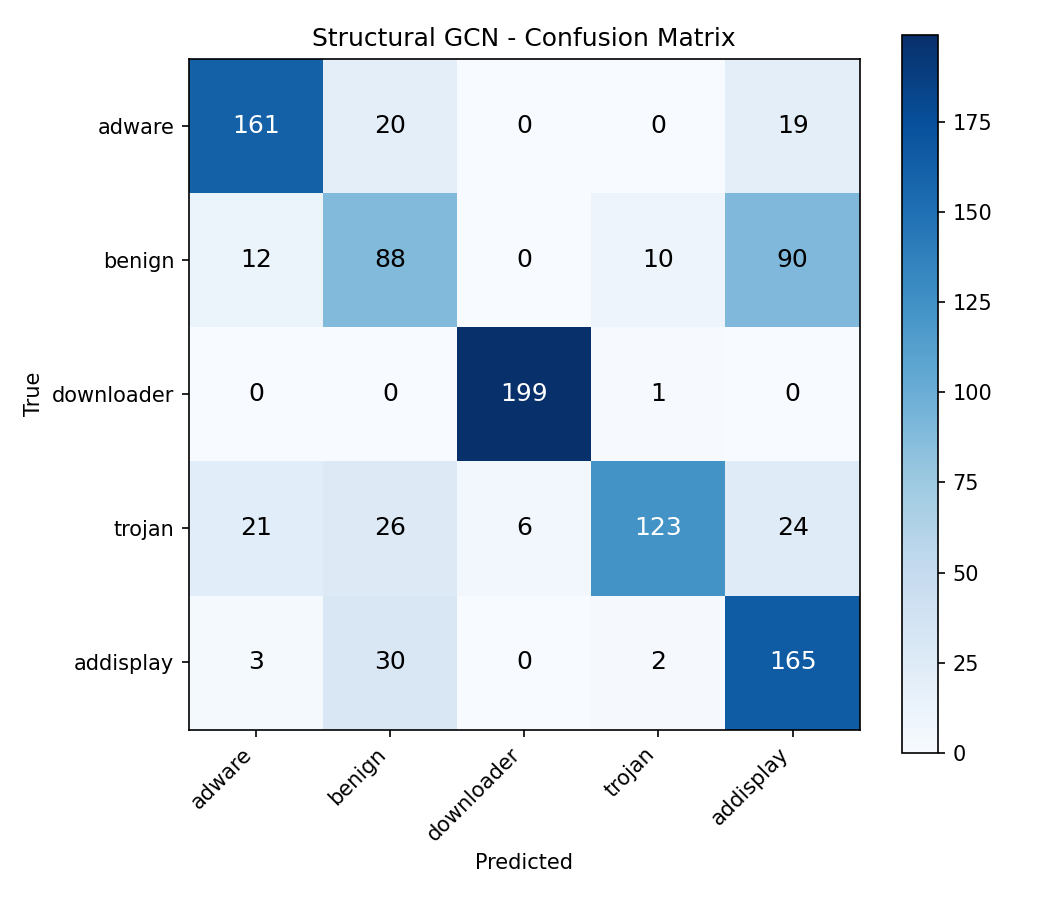
\includegraphics[width=0.6\linewidth]{figures/baseline_structural_confusion_matrix.png}
    \caption{Confusion matrix for the structural GCN on the standard test split. }
    \label{fig:structural_cm}
\end{figure}

\begin{figure}[h]
    \centering
    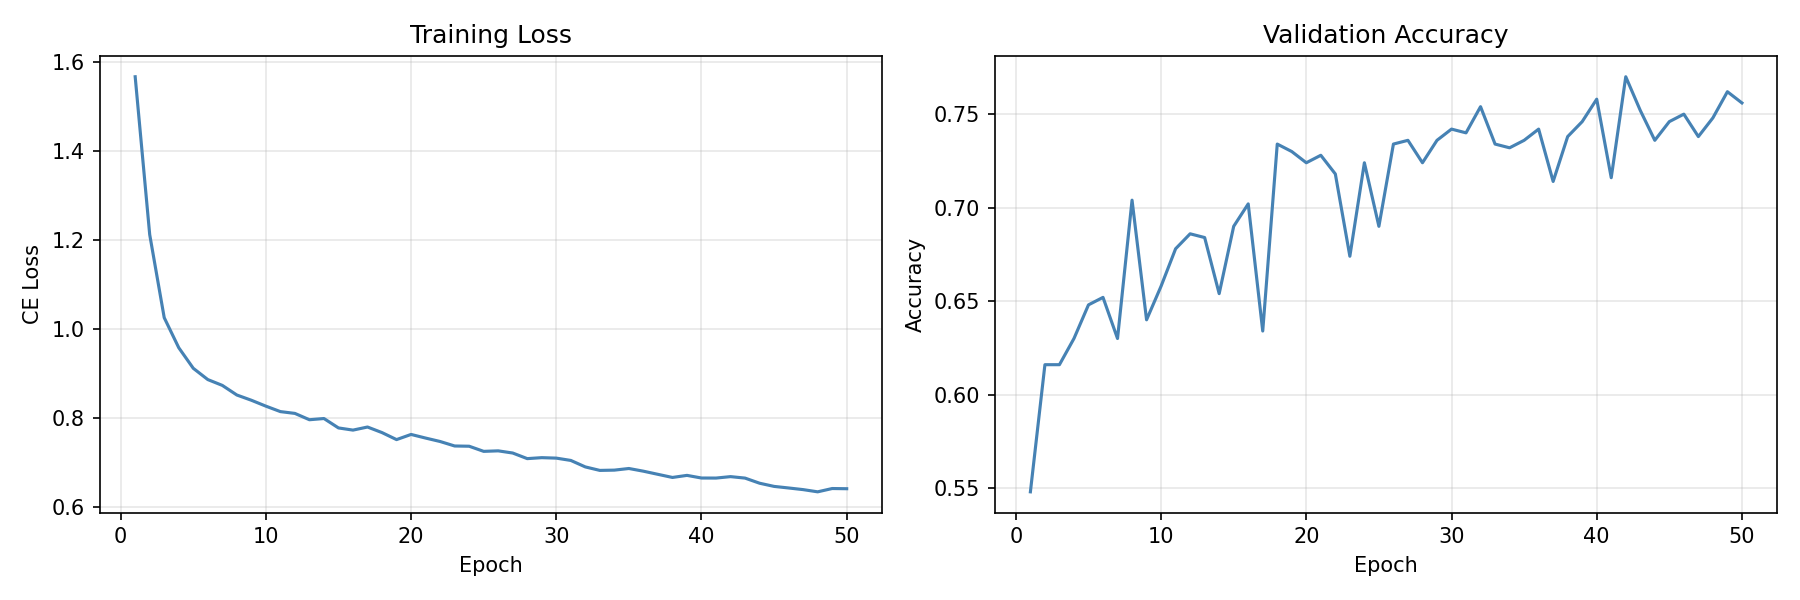
\includegraphics[width=0.8\linewidth]{figures/baseline_structural_training_curve.png}
    \caption{Training loss and validation accuracy curves for the structural GCN. }
    \label{fig:structural_curves}
\end{figure}

\subsubsection{Phase 2 observations}

\begin{itemize}
    \item Both EnrichedGCN methods gave similar results, with zero-fill at 0.737 and prune at 0.738, which is close to the structural baseline (0.746). This is expected since the semantic features mainly help under distribution shift. 
    \item Prune trained better than zero-fill in terms of loss, but both had similar test accuracy. 
    \item The individual class results were similar to phase 1, with great performance on downloader and poor performance on benign, along with confusion between similar classes.
\end{itemize}

\begin{figure}[h]
    \centering
    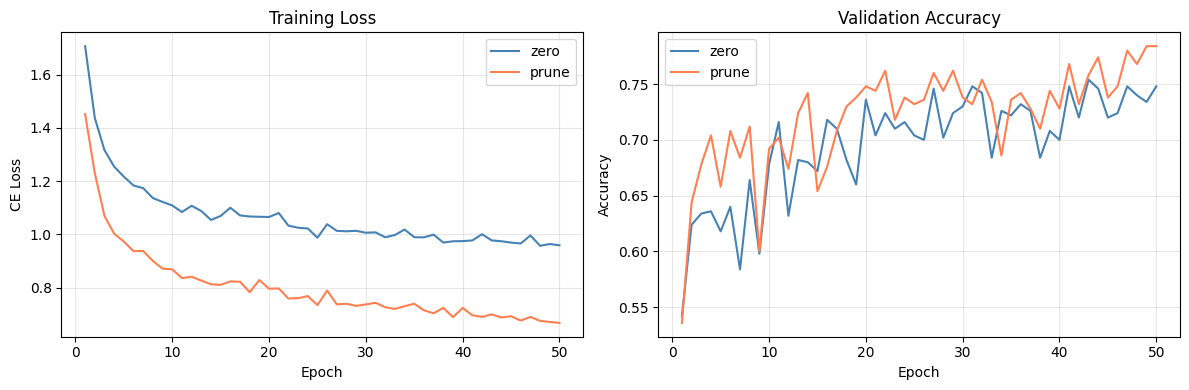
\includegraphics[width=0.8\linewidth]{figures/enriched_compare_curves.png}
    \caption{Training loss and validation accuracy for EnrichedGCN under zero-fill and prune. }
    \label{fig:enriched_curves}
\end{figure}

\subsubsection{Phase 3 observations}

\begin{itemize}
    \item GatedGCN had a 71.7\% accuracy, slightly below the other models which had a range from 73.7 to 74.6\%. On the standard split, it did not improve over EnrichedGCN, since all features are present and the gate had little effect. 
    \item The gate output changed across different mask inputs, so the model was using the missingness mask, but this effect was not important enough to improve accuracy.
    \item The individual class results were similar to earlier phases, with some improvement on benign and a poorer performance on addisplay, along with confusion between similar classes. 
\end{itemize}

\begin{figure}[h]
    \centering
    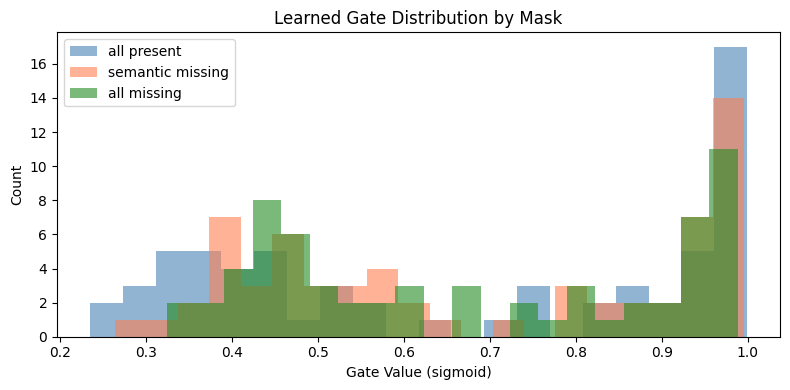
\includegraphics[width=0.7\linewidth]{figures/gated_weights_histogram.png}
    \caption{Learned gate distribution for different mask inputs. }
    \label{fig:gating_hist}
\end{figure}

\begin{figure}[h]
    \centering
    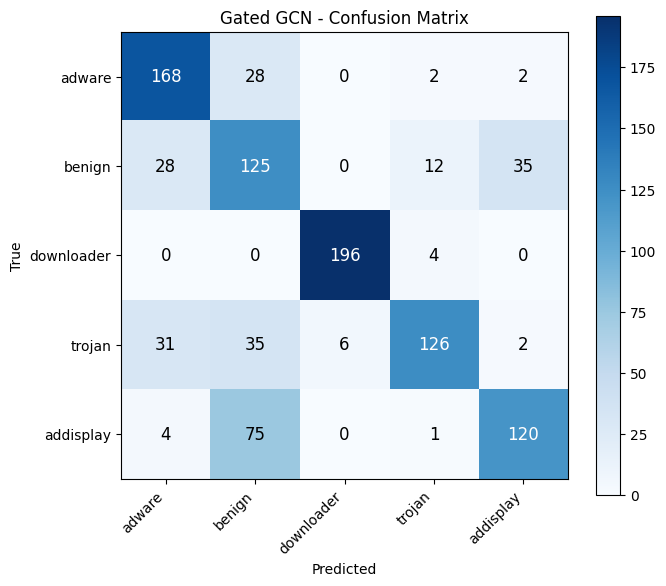
\includegraphics[width=0.6\linewidth]{figures/gated_confusion_matrix.png}
    \caption{Confusion matrix for GatedGCN on the standard test split. }
    \label{fig:gated_cm_standard}
\end{figure}

\begin{figure}[h]
    \centering
    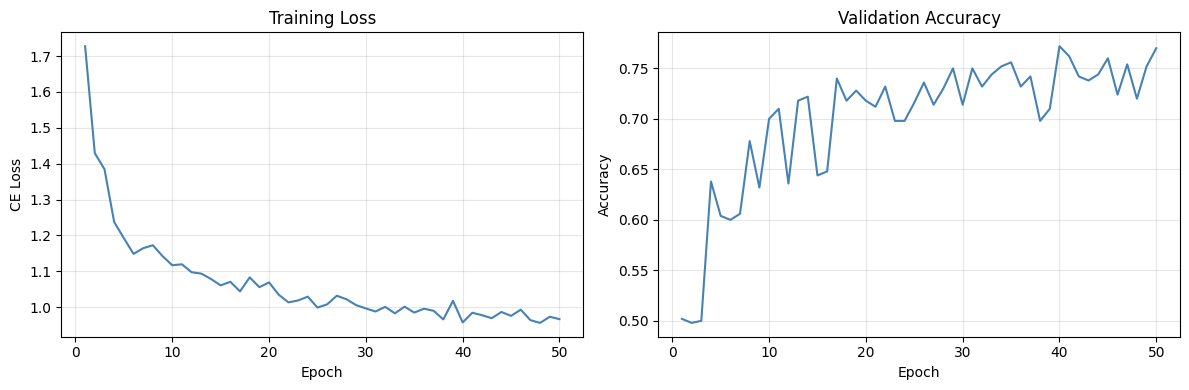
\includegraphics[width=0.8\linewidth]{figures/gated_training_curve.png}
    \caption{Training loss and validation accuracy curves for GatedGCN.}
    \label{fig:gated_curves}
\end{figure}

\subsection{Shifted Split (MalNet-Tiny-Common)}

\begin{itemize}
    \item This table shows what happens when the same trained models are evaluated on Tran et al.'s Common shifted test split.
\end{itemize}

\begin{table}[h]
\centering
\begin{tabular}{lccc}
\hline
\textbf{Model} & \textbf{Standard Accuracy} & \textbf{Shifted Accuracy} & \textbf{Robustness Gap} \\
\hline
Structural GCN & 0.7460 & 0.3840 & 0.3620 \\
Enriched GCN (zero-fill) & 0.7370 & 0.4120 & 0.3250 \\
Enriched GCN (prune) & 0.7380 & 0.4280 & 0.3100 \\
Gated GCN & 0.7170 & 0.3800 & 0.3370 \\
\hline
\end{tabular}
\caption{Shifted split results and robustness gap.}
\label{tab:shifted_results}
\end{table}

\begin{figure}[h]
    \centering
    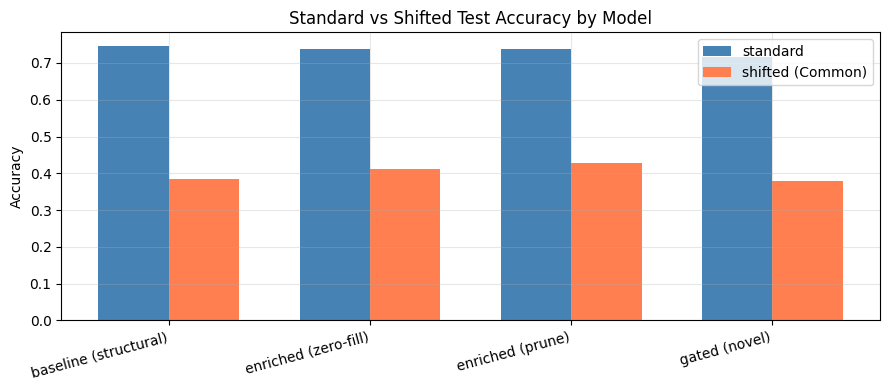
\includegraphics[width=0.7\linewidth]{figures/robustness_gap_bar_graph.png}
    \caption{Standard versus shifted accuracy for all models.}
    \label{fig:robustness_gap_bar}
\end{figure}

\subsubsection{Phase 4 observations}

\begin{itemize}
    \item The structural baseline had the largest robustness gap (0.3620), while EnrichedGCN with zero-fill and prune reduced it to 0.3250 and 0.3100. This shows that adding semantic features and training with missingness improved robustness.
    \item The GatedGCN model did not improve on the simpler EnrichedGCN variants. Its robustness gap was 0.3370, which is better than the structural baseline, but worse than both EnrichedGCN models.
    \item On the shifted set, the confusion matrix shows that the model made different mistakes than on the standard split. This can be seen with adware, benign, and downloader. This shows that the Common split I used created a real distribution shift.
\end{itemize}

\subsection{Comparison with Tran et al. [1]}

\begin{itemize}
    \item This table compares my results against the reference paper's numbers.
\end{itemize}

\begin{table}[h]
\centering
\begin{tabular}{lccc}
\hline
\textbf{Source} & \textbf{Features} & \textbf{Pooling} & \textbf{Standard Accuracy} \\
\hline
GCN (one hot degree) & one hot degree & mean & 0.7510 \\
Structural GCN & LDP + synthetic & mean & 0.7460 \\
GCN (Tran et al. [1]) & LDP & max & 0.856 \\
GIN (Tran et al. [1]) & LDP & max & 0.912 \\
GCN (semantic features from Tran et al. [1]) & metadata + LLM + LDP & max & 0.935 \\
\hline
\end{tabular}
\caption{Comparison with Tran et al. [1] on the standard split.}
\label{tab:tran_compare}
\end{table}

\begin{itemize}
    \item The difference between my structural GCN (74.6\%) and Tran et al.'s GCN with LDP (85.6\%) is expected [1]. Their model uses max pooling, while mine uses mean pooling and synthetic features. 
\end{itemize}

\section{Discussion}

\begin{itemize}
    \item With the standard split, the one hot degree baseline still performed slightly better than the new variants, so the added features did not improve test accuracy. 
    \item The shifted split shows another difference, because the robustness gap drops from 0.3620 (structural baseline) to 0.3250 and 0.3100 for the enriched GCN models, showing improvement in robustness. 
    \item The GatedGCN did not improve over the EnrichedGCN models. Its gap (0.3370) was better than the baseline but worse than both enriched versions. 
    \item The most likely reason is that the synthetic semantic features were not important enough for the gate to use effectively. Real APK metadata would have given a better result, I feel. 
\end{itemize}

\section{Limitations}

\begin{itemize}
    \item Tran et al. [1] used real APK metadata, while I used synthetic features due to computational limits. This affects the accuracy, but comparisons between my models are still useful.
    \item I used mean pooling and a simpler training setup, while Tran et al. used max pooling, which may have affected performance. 
    \item Some features were skipped for graphs with more than 4,000 nodes due to memory limits, so those graphs may have weaker features.
\end{itemize}

\section{Future Work}

\begin{itemize}
    \item The next step would be to use the real Tran et al. [1] metadata without the LLM embeddings and rerun the gating experiment with better semantic features.
    \item Adding GIN and other model types would help determine if the gating result depends on the model structure.
\end{itemize}

\section{Conclusion}

\begin{itemize}
    \item The main finding is that EnrichedGCN with prune handling had the smallest robustness gap, reducing it from 0.3620 to 0.3100. I showed that adding semantic features and training with missingness can improve robustness under distribution shift, but perhaps this would have been more conclusive with the actual data. 
    
    \item The GatedGCN model did not improve further, probably because of the synthetic features.
    
    \item Overall, I learned about more deep learning methodology and malware in machine learning. I learned simple feature enrichment and training strategies can improve robustness, but more meaningful semantic features would likely lead to better results.
\end{itemize}



\begin{thebibliography}{9}

\bibitem{tran2025}
Tran et al.,
``Mitigating Distribution Shift in Graph-Based Android Malware Classification via Function Metadata and LLM Embeddings,''
arXiv preprint arXiv:2508.06734, 2025. [Online]. Available: \url{https://arxiv.org/html/2508.06734v1}

\bibitem{freitas2020malnet}
S. Freitas, Y. Dong, J. Neil, and D. H. Chau,
``A Large-Scale Database for Graph Representation Learning,''
in \textit{Proceedings of the NeurIPS Track on Datasets and Benchmarks}, 2021. [Online]. Available: \url{https://openreview.net/forum?id=1xDTDk3XPW}

\bibitem{kipf2017gcn}
T. N. Kipf and M. Welling,
``Semi-Supervised Classification with Graph Convolutional Networks,''
in \textit{International Conference on Learning Representations (ICLR)}, 2017. [Online]. Available: \url{https://arxiv.org/abs/1609.02907}

\bibitem{fey2019pyg}
M. Fey and J. E. Lenssen,
``Fast Graph Representation Learning with PyTorch Geometric,''
in \textit{ICLR Workshop on Representation Learning on Graphs and Manifolds}, 2019. [Online]. Available: \url{https://arxiv.org/abs/1903.02428}

\bibitem{cai2018ldp}
C. Cai and Y. Wang,
``A Simple yet Effective Baseline for Non-attributed Graph Classification,''
arXiv preprint arXiv:1811.03508, 2018. [Online]. Available: \url{https://arxiv.org/abs/1811.03508}

\bibitem{nntvuhf}
N. N. Tran,
``MalNet-Tiny-Features,'' Hugging Face Datasets, 2025. [Online]. Available: \url{https://huggingface.co/datasets/nntvu/MalNet-Tiny-Features}

\bibitem{hamilton2017graphsage}
W. L. Hamilton, R. Ying, and J. Leskovec,
``Inductive Representation Learning on Large Graphs,''
in \textit{Advances in Neural Information Processing Systems (NeurIPS)}, vol. 30, 2017, pp. 1024--1034. [Online]. Available: \url{https://arxiv.org/abs/1706.02216}

\bibitem{quinonero2009datasetshift}
J. Qui\~nonero-Candela, M. Sugiyama, A. Schwaighofer, and N. D. Lawrence, Eds.,
\textit{Dataset Shift in Machine Learning}.
Cambridge, MA: MIT Press, 2009. [Online]. Available: \url{https://direct.mit.edu/books/edited-volume/3841/Dataset-Shift-in-Machine-Learning}

\end{thebibliography}

\end{document}
